\section{Experiments}

We have implemented a tool chain that takes as input a description
of the polytopes in terms of vertices, and the parallelepiped boundaries,
and it returns the placement vectors for the arrangement, if any
exists.

In order to compute the facets of the polytopes we rely on the CGAL 
library~\cite{CGAL}. We then solve the SMT problem with some
efficient and open-source SMT-solver, such as CVC4~\cite{CVC4}, OpenSMT~\cite{OpenSMT}, 
or Z3~\cite{Z3}. We use CGAL again
to export the solution returned by the SMT-Solver into the VRML graphical models
that can be seen in this paper. The source code of our tool-chain can 
be downloaded from~\url{https://github.com/bobosoft/polytopepacking}. 
At the same address it is possible to obtain the problem descriptions, the
encoded smt2 files, and the 3D models of the results.

As an experiment to test our proof-of-concept tool-chain we have
encoded and solved the first problem described in~\cite{sto03}, where
7 polytopes are placed in a parallelepiped of length 12 and width 10.
\cite{sto03} shows a placement of height 27, which is a local optima for
the approach of that paper. By running our tool-chain we were able to
prove, in about 10 minutes, that a height of 23 is actually sufficient.
We were not able to obtain a model for height 22 within an hour, and
the polytope placement is shown in Figure~\ref{fig:p7}. In these
trials we have increased and decreased the value for the height manually,
but this process can be automated in a way that is standard among
optimizing solvers.

A more automated implementation, and more exhaustive and detailed 
experimentation are left as future work.

%% \begin{figure}
%% \begin{center}
%% \begin{tabular}{cccc}
%% \begin{minipage}{.2\textwidth}
%% 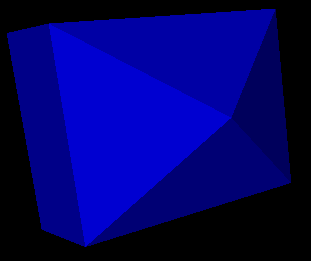
\includegraphics[scale=.2]{poly_1.png}
%% \end{minipage}
%% &
%% \begin{minipage}{.2\textwidth}
%% 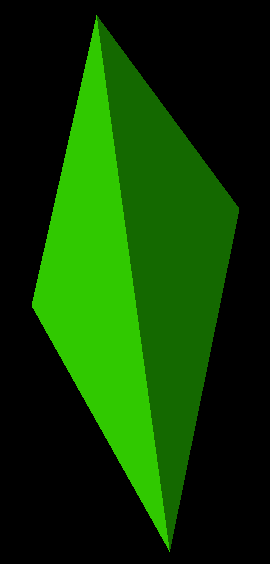
\includegraphics[scale=.2]{poly_2.png}
%% \end{minipage}
%% &
%% \begin{minipage}{.2\textwidth}
%% 
\includegraphics[scale=.2]{poly_3.png}
%% \end{minipage}
%% &
%% \begin{minipage}{.2\textwidth}
%% 
\includegraphics[scale=.2]{poly_4.png}
%% \end{minipage}
%% \\
%% \begin{minipage}{.2\textwidth}
%% 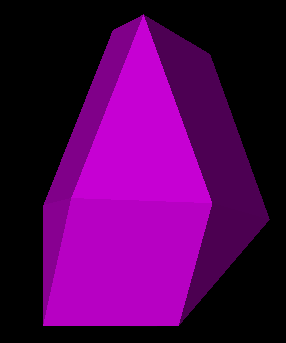
\includegraphics[scale=.2]{poly_5.png}
%% \end{minipage}
%% &
%% \begin{minipage}{.2\textwidth}
%% 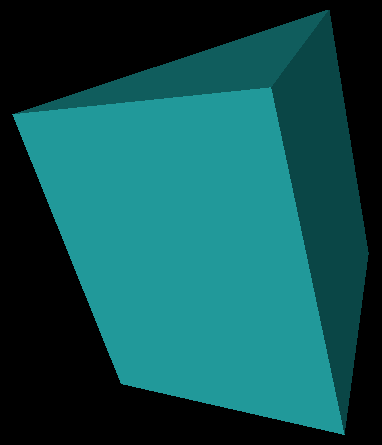
\includegraphics[scale=.2]{poly_6.png}
%% \end{minipage}
%% &
%% \begin{minipage}{.2\textwidth}
%% 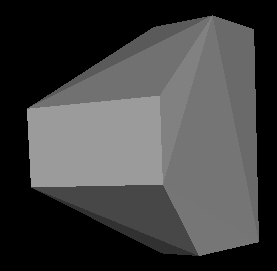
\includegraphics[scale=.2]{poly_7.png}
%% \end{minipage}
%% \end{tabular}
%% \end{center}
%% \caption{The polytopes that are to be packed.}
%% \label{fig:p}
%% \end{figure}

\begin{figure}
\begin{center}
\begin{tabular}{cc}
\begin{minipage}{.4\textwidth}
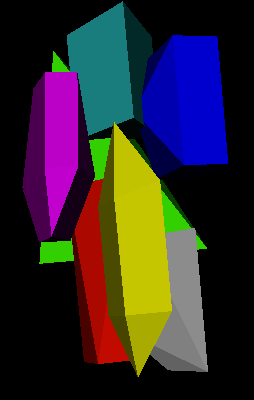
\includegraphics[scale=.5]{problem_7_1.png}
\end{minipage}
&
\begin{minipage}{.4\textwidth}
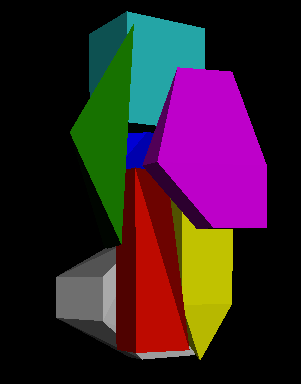
\includegraphics[scale=.5]{problem_7_2.png}
\end{minipage}
\end{tabular}
\end{center}
\caption{Two views of the packing placement for 7 polytopes as per~\cite{sto03} 
for a height of 23.}
\label{fig:p7}
\end{figure}
